% =====================================================================
%  Figure captions for: A Unary Admissibility Predicate for Molecular
%  Comparison
%
%  Every quantity quoted below is read from
%  validation/results/exp_unary.json and exp_conservation.json.
%  All minimum cuts are exact (maximum flow), so no agreement reported
%  here can be a solver artefact.
% =====================================================================

\begin{figure*}[!htbp]
    \centering
    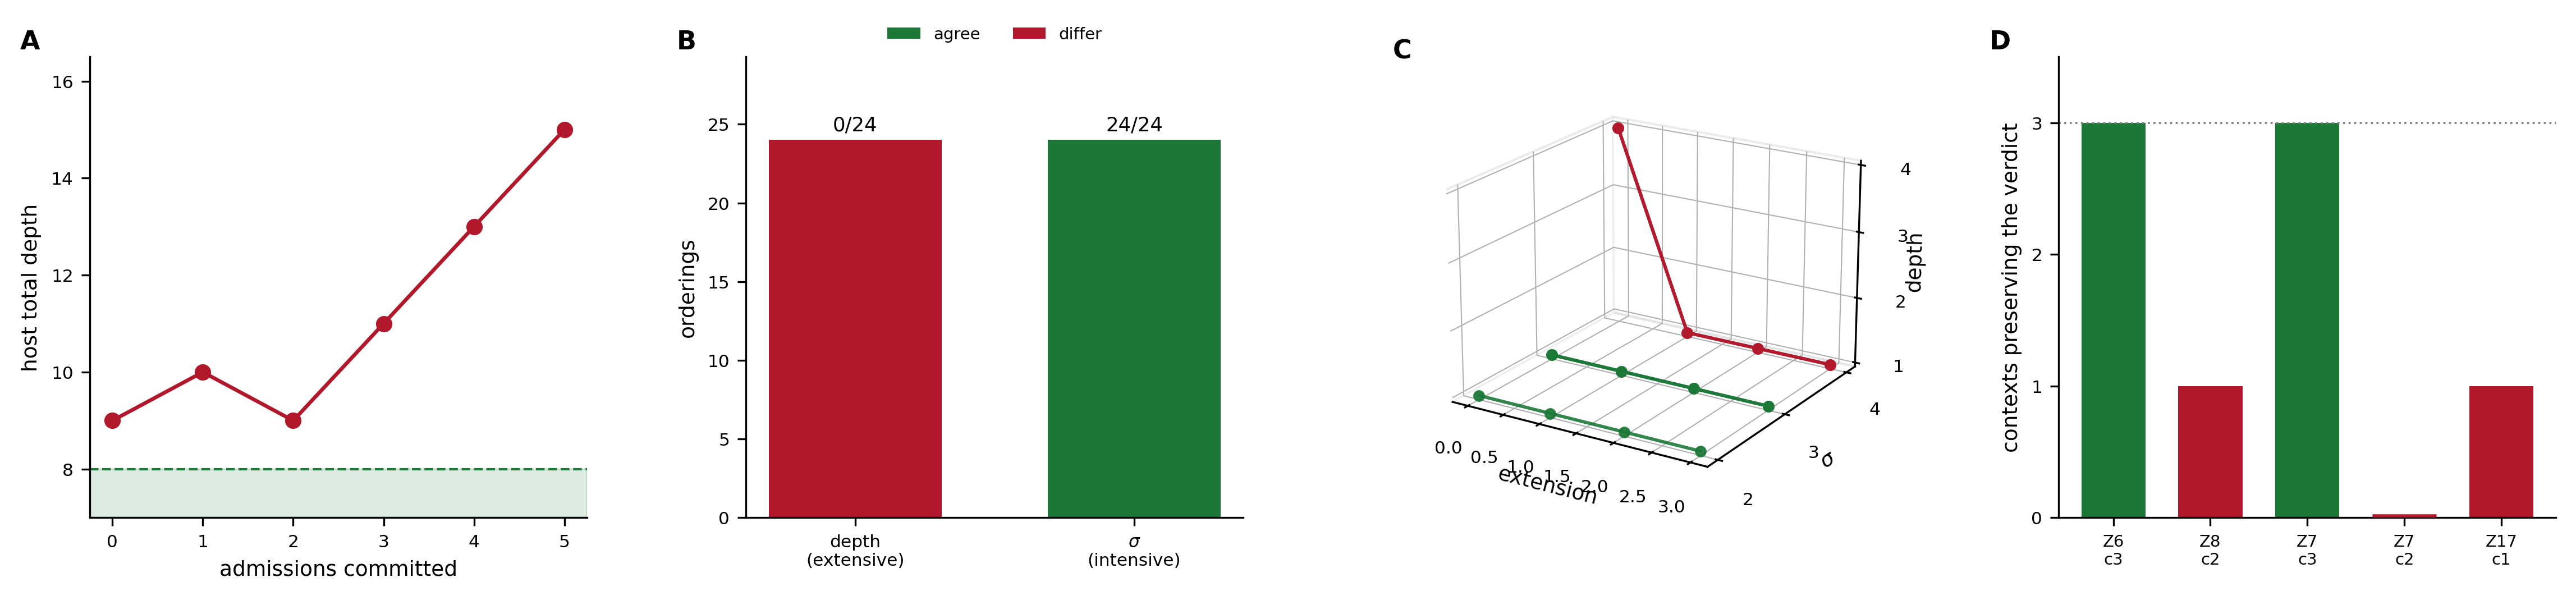
\includegraphics[width=\textwidth]{figures/panel_01_extensive_fails.png}
    \caption{\textbf{A window on an extensive functional is not a unary
    predicate: the verdict depends on what has already been admitted, and
    every one of $24$ orderings disagrees with the canonical answer.}
    All quantities are computed on contact graphs (\Cref{def:graph}) whose
    separation costs are exact minimum cuts (\Cref{def:key}), so the
    failure below is a property of the construction rather than of a
    tolerance or a solver.
    (\textbf{A})~The host's total depth against the number of admissions
    committed, with the calibrated window $[7,8]$ shaded. The bare host
    already sits at $9$, above the window, and successive admissions carry
    it to $10,9,11,13,15$ --- rising by two per admission once the first
    is past. This is \Cref{thm:extensive-fails} in its measured form: a
    bounded window on an eventually-monotone quantity closes after a
    bounded number of admissions, and here the bound is one.
    (\textbf{B})~Orderings agreeing with the canonical admissible set, for
    a window on total depth against a window on the inserted node's own
    $\sep$. The extensive window agrees on $0$ of $24$; the intensive one
    on $24$ of $24$. The bars are stacked rather than overlaid because an
    agreement count of zero would otherwise be an invisible bar and read
    as missing data rather than as total failure.
    (\textbf{C})~The local key $(\sep,\dep)$ of each of the five distinct
    candidates traced across four successive extensions of the host. Every
    trajectory is flat in $\sep$; two are flat in $\dep$ and two drop from
    $\dep=4$ to $\dep=1$ at the first extension. The two components of the
    cut key are therefore not interchangeable, which is the measurement
    \Cref{thm:sigma-intensive} rests on.
    (\textbf{D})~For each candidate, how many of the three tested contexts
    preserved its bare-host verdict under the extensive window. Two
    candidates survive all three and three survive none; the aggregate is
    the context agreement of $0.400$ reported in \Cref{tab:round1}. A
    candidate's verdict changing with context is precisely the violation
    of \Cref{def:unary}.}
    \label{fig:extensive}
\end{figure*}

\begin{figure*}[!htbp]
    \centering
    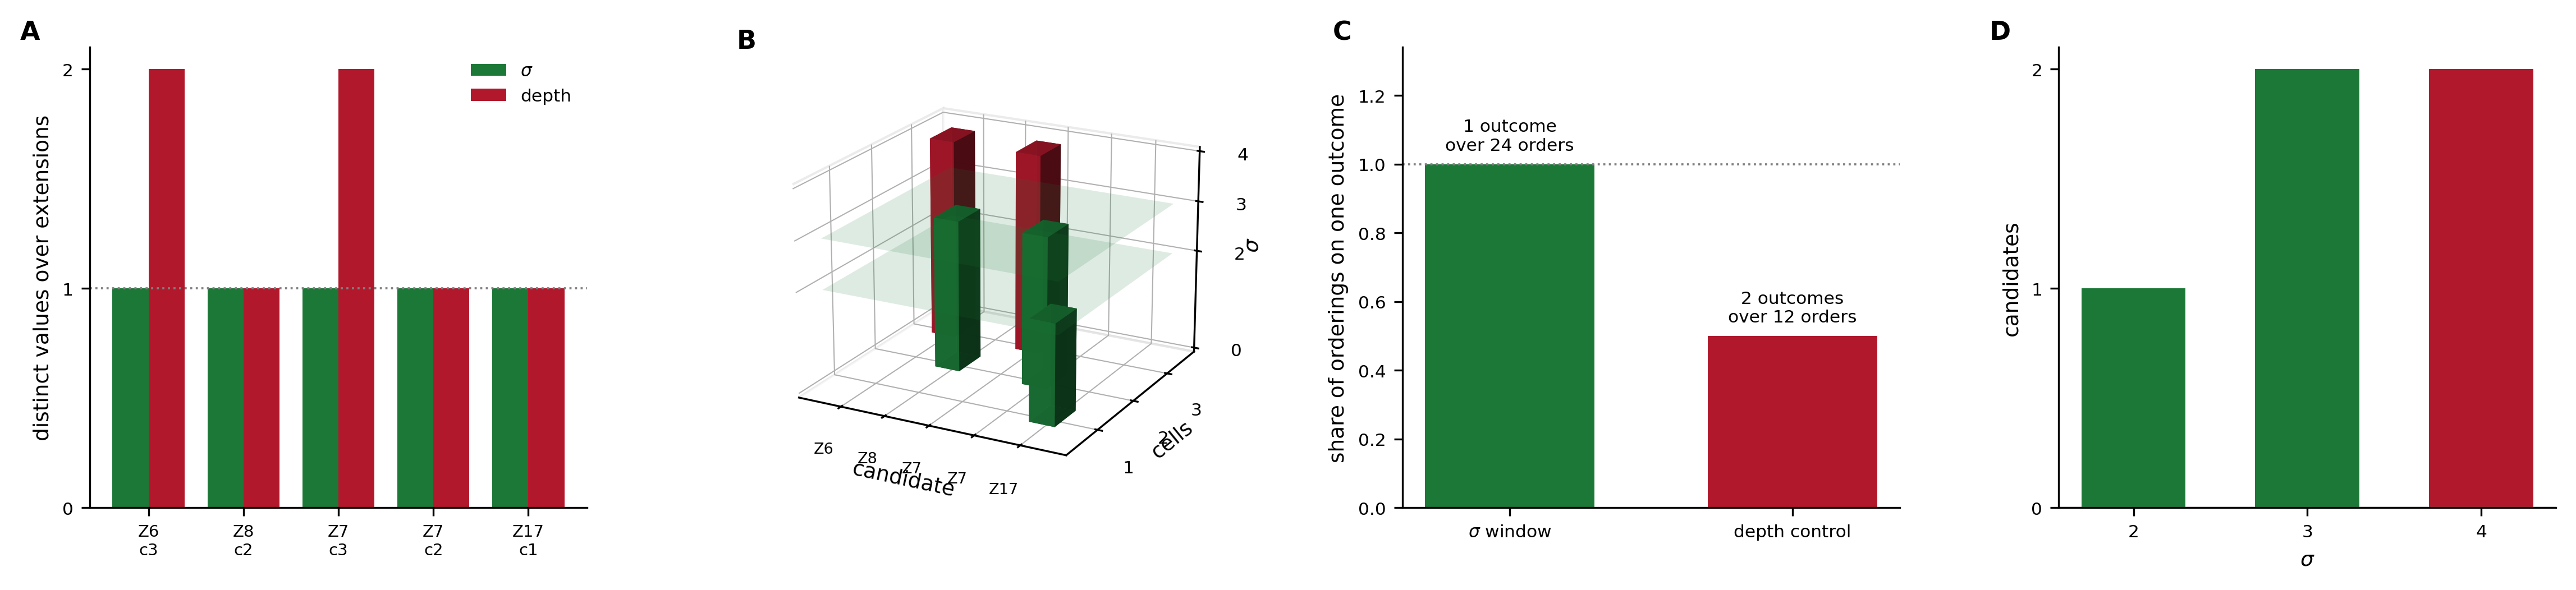
\includegraphics[width=\textwidth]{figures/panel_02_intensive_works.png}
    \caption{\textbf{A window on $\sep$ alone is order independent in all
    $24$ orderings and admits $0.600$ of the pool, while the same
    construction on $\dep$ is order dependent --- which is what makes the
    $\sep$ result a claim about $\sep$ and not about the harness.}
    (\textbf{A})~Distinct values taken by each key component across four
    extensions, per candidate. $\sep$ takes one value for all five
    candidates; $\dep$ takes two for the two three-cell candidates. The
    dotted line at $1$ is the stability threshold: a bar above it is a
    component that moved when the graph grew elsewhere.
    (\textbf{B})~The admission rule in three dimensions. Bar height is the
    candidate's own $\sep$ and the translucent slab is the window
    $[2.0,3.0]$; green bars terminate inside it and red bars rise through
    it. Height is $\sep$ rather than a $0/1$ verdict deliberately --- a
    verdict-height plot would render every rejected candidate as a
    zero-height, invisible bar, hiding exactly the cases that carry the
    result.
    (\textbf{C})~Share of orderings landing on a single outcome, for the
    $\sep$ window against the $\dep$ control. The $\sep$ window reaches
    $1.000$ over $24$ orderings; the control reaches $0.500$, producing
    two distinct outcomes over $12$. The axis is a share rather than a
    count of distinct outcomes so that taller means better and the two
    bars sit on one scale.
    (\textbf{D})~Candidates at each observed $\sep$ value, coloured by
    whether the window admits them. Three of five candidates fall in
    $\{2.0,3.0\}$ and two at $4.0$, giving the admissible fraction of
    $0.600$ reported in \Cref{tab:round2}. A window admitting everything
    or nothing would classify nothing, so this non-vacuity is a
    precondition for the result rather than an ornament.}
    \label{fig:intensive}
\end{figure*}

\begin{figure*}[!htbp]
    \centering
    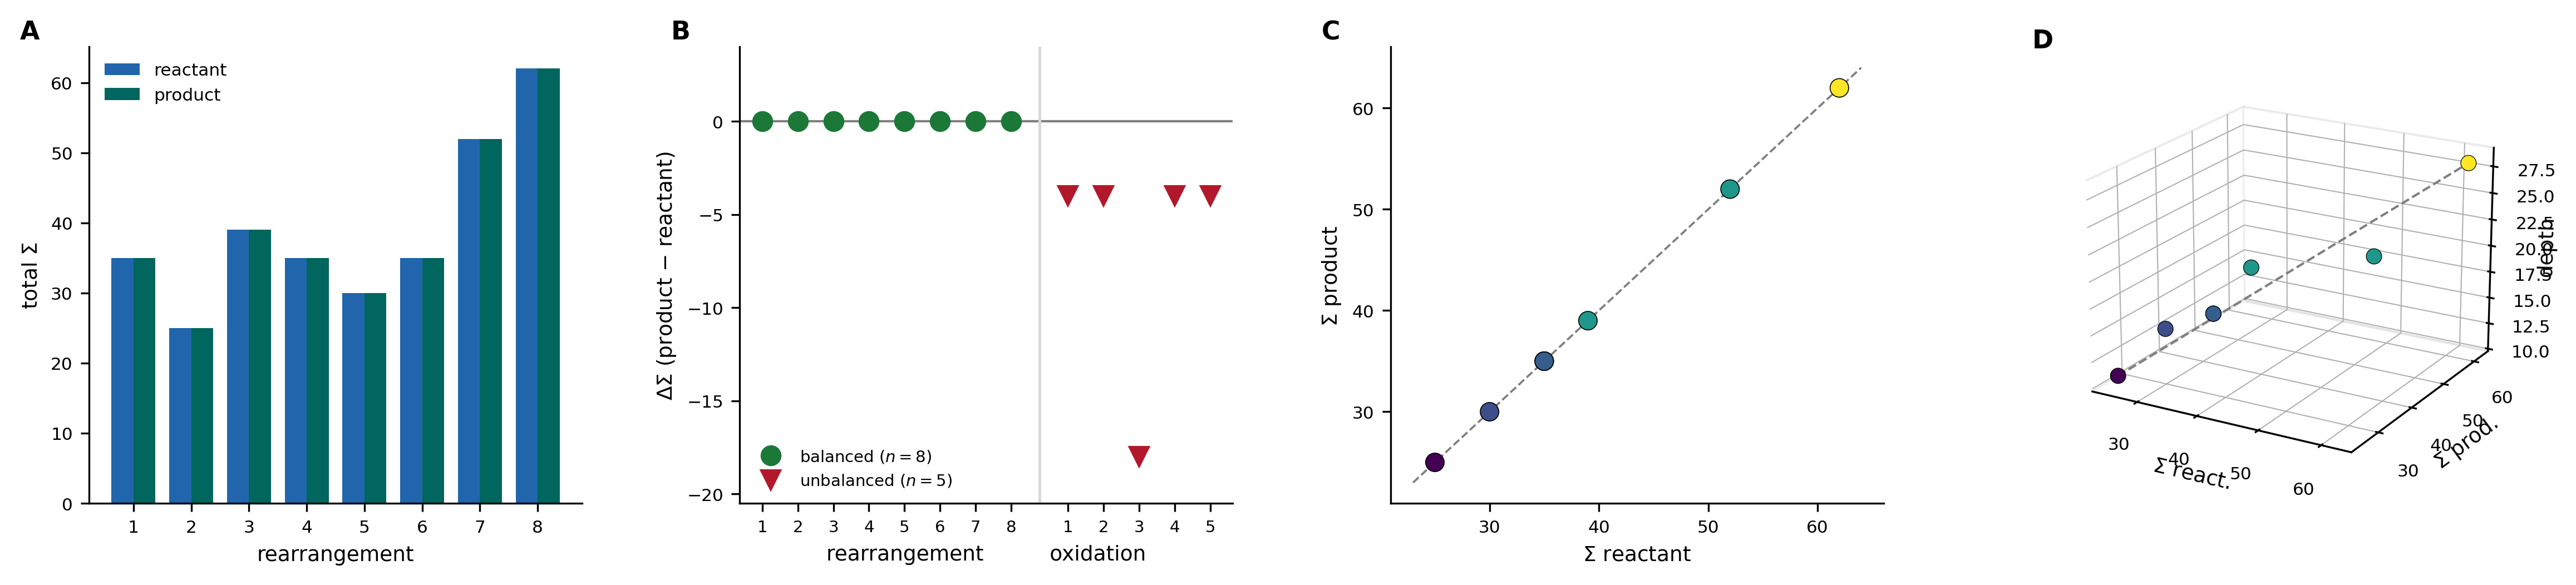
\includegraphics[width=\textwidth]{figures/panel_03_conservation.png}
    \caption{\textbf{Total cut weight is exactly conserved across all
    eight balanced rearrangements, and moves on every one of five
    unbalanced controls.}
    A balanced rearrangement (\Cref{def:balanced}) has the same multiset of
    atoms on both sides, hydrogens included; the controls are oxidations,
    which differ by $\mathrm{H}_2$ and are therefore not rearrangements.
    (\textbf{A})~Total $\Sigma$ for reactant and product of each balanced
    pair. The two bars coincide exactly in all eight cases. The corpus
    spans $\Sigma$ from $25$ to $62$, so the agreement is not an artefact
    of a narrow range.
    (\textbf{B})~Residual $\Delta\Sigma$ for the balanced set (green,
    left) against the unbalanced controls (red, right). The balanced
    residuals are identically zero; the controls run from $-4.0$ to
    $-18.0$. Plotting the two together is what makes the flat green line
    informative: a quantity that never moves is indistinguishable, in a
    results file, from one that is not being computed, and the controls
    show it is capable of moving.
    (\textbf{C})~$\Sigma$ product against $\Sigma$ reactant with the
    identity line drawn, points coloured by total depth. All eight lie on
    the diagonal.
    (\textbf{D})~The same pairs in $(\Sigma_{\text{react}},
    \Sigma_{\text{prod}},\text{depth})$ space with the identity line. The
    points lie on the diagonal plane in both coordinates simultaneously:
    depth is conserved on the same eight pairs, $8/8$ exactly, so the
    conservation is not specific to the cut weight.}
    \label{fig:conservation}
\end{figure*}

\begin{figure*}[!htbp]
    \centering
    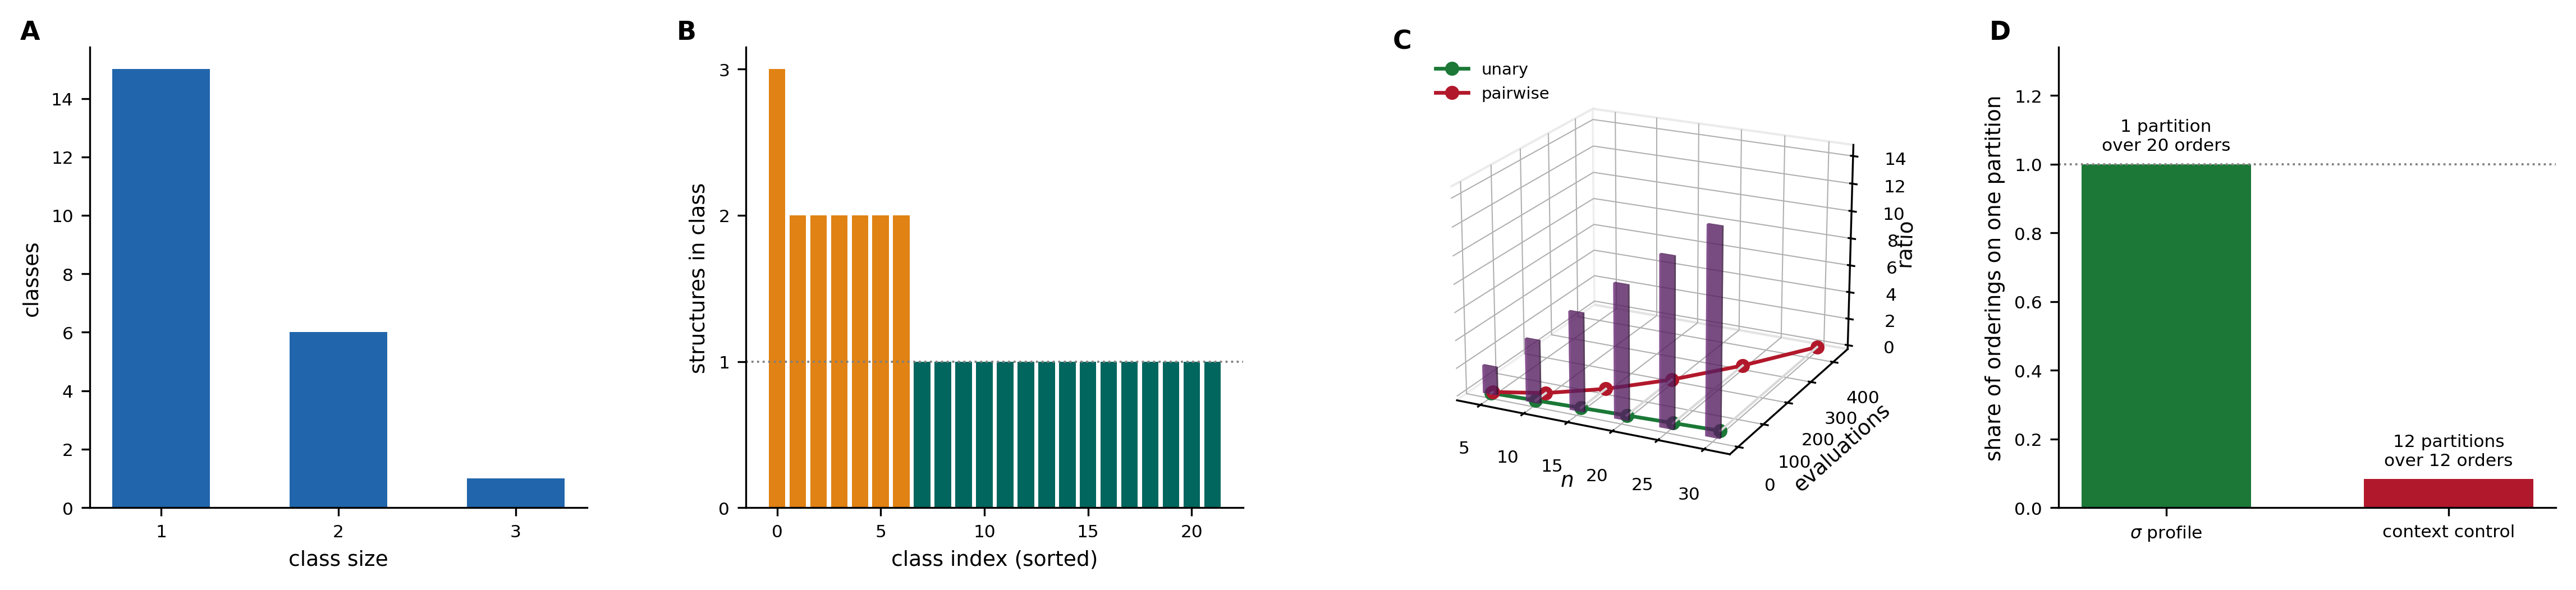
\includegraphics[width=\textwidth]{figures/panel_04_corpus.png}
    \caption{\textbf{At corpus scale the $\sep$ profile yields $22$
    classes over $30$ structures, identically under $20$ shuffles, against
    a context-reading control that differs under all $12$ of its
    orderings.}
    (\textbf{A})~Distribution of class sizes: $15$ singletons, $6$ classes
    of two, and one class of three. That the tail is this short is what
    makes the profile a usable screen; that it is not empty is why
    \Cref{rem:not-identity} insists the profile is not an identity test.
    (\textbf{B})~Class occupancy sorted by size, singletons in teal and
    multi-structure classes in orange. Neither one class nor thirty ---
    the screen discriminates, which is the condition
    \Cref{def:profile} needs to be worth computing.
    (\textbf{C})~The counting law of \Cref{prop:counting}. Unary
    evaluations (green) and pairwise comparisons (red) against corpus
    size, with the ratio drawn as bars on the third axis, reaching $14.5$
    at $n=30$. The identity $\binom{n}{2}/n=(n-1)/2$ holds exactly at
    every point measured. This is a count of evaluations and not a
    timing; \Cref{rem:not-speedup} states what it does and does not mean.
    (\textbf{D})~Share of orderings landing on a single partition, for the
    $\sep$ profile against a control whose key reads accumulated context.
    The profile reaches $1.000$ over $20$ shuffles; the control reaches
    $1/12$, producing a different partition under every ordering. Without
    a control that fails, panel~(\textbf{D})'s left bar would be
    consistent with an implementation that ignores its input entirely.}
    \label{fig:corpus}
\end{figure*}
